% \documentclass[handout]{beamer}
\documentclass{beamer}

\mode<presentation>
{
  \usetheme{default}
  \usefonttheme[onlymath]{serif}
  % \usetheme{Singapore}
  % \usetheme{Warsaw}
  % \usetheme{Malmoe}
  % \useinnertheme{circles}
  % \useoutertheme{infolines}
  % \useinnertheme{rounded}

  \setbeamercovered{transparent=20}
}

\usepackage[english]{babel}
\usepackage[latin1]{inputenc}
\usepackage{alltt,listings,multirow,ulem,siunitx}
\usepackage[absolute,overlay]{textpos}
\TPGrid{1}{1}
\usepackage{pdfpages}
\usepackage{multimedia}
\usepackage{multicol}
\newcommand\hmmax{0}
\newcommand\bmmax{0}
\usepackage{bm}
\usepackage{comment}

% font definitions, try \usepackage{ae} instead of the following
% three lines if you don't like this look
\usepackage{mathptmx}
\usepackage[scaled=.90]{helvet}
% \usepackage{courier}
\usepackage[T1]{fontenc}
\usepackage{tikz}
\usetikzlibrary{decorations.pathreplacing}
\usetikzlibrary{shadows,arrows,shapes.misc,shapes.arrows,shapes.multipart,arrows,decorations.pathmorphing,backgrounds,positioning,fit,petri,calc,shadows,chains,matrix}


% \usepackage{pgfpages}
% \pgfpagesuselayout{4 on 1}[a4paper,landscape,border shrink=5mm]

\usepackage{JedMacros}

\newcommand{\timeR}{t_{\mathrm{R}}}
\newcommand{\timeW}{t_{\mathrm{W}}}
\newcommand{\mglevel}{\ensuremath{\ell}}
\newcommand{\mglevelcp}{\ensuremath{\mglevel_{\mathrm{cp}}}}
\newcommand{\mglevelcoarse}{\ensuremath{\mglevel_{\mathrm{coarse}}}}
\newcommand{\mglevelfine}{\ensuremath{\mglevel_{\mathrm{fine}}}}

%solution and residual
\newcommand{\vx}{\ensuremath{x}}
\newcommand{\vc}{\ensuremath{\hat{x}}}
\newcommand{\vr}{\ensuremath{r}}
\newcommand{\vb}{\ensuremath{b}}

%operators
\newcommand{\vA}{\ensuremath{A}}
\newcommand{\vP}{\ensuremath{I_H^h}}
\newcommand{\vS}{\ensuremath{S}}
\newcommand{\vR}{\ensuremath{I_h^H}}
\newcommand{\vI}{\ensuremath{\hat I_h^H}}
\newcommand{\vV}{\ensuremath{\mathbf{V}}}
\newcommand{\vF}{\ensuremath{F}}
\newcommand{\vtau}{\ensuremath{\mathbf{\tau}}}


\title{GPU-accelerated smoothed aggregation algebraic multigrid: Multi-node scalability and versatility}
\author{{\bf Jed Brown}\inst{1} and Steven Dalton\inst{2} \\
  {\small thanks to Karl Rupp\inst{1} and Luke Olson\inst{2}}}

% - Use the \inst command only if there are several affiliations.
% - Keep it simple, no one is interested in your street address.
\institute
{
  \inst{1}{Mathematics and Computer Science Division, Argonne National Laboratory} \\
  \inst{2}{Department of Computer Science, University of Illinois at Urbana-Champaign}
}

\date{GPU-SMP, Changchun, 2013-07-30}

% This is only inserted into the PDF information catalog. Can be left
% out.
\subject{Talks}


% If you have a file called "university-logo-filename.xxx", where xxx
% is a graphic format that can be processed by latex or pdflatex,
% resp., then you can add a logo as follows:

% \pgfdeclareimage[height=0.5cm]{university-logo}{university-logo-filename}
% \logo{\pgfuseimage{university-logo}}



% Delete this, if you do not want the table of contents to pop up at
% the beginning of each subsection:
% \AtBeginSubsection[]
% {
% \begin{frame}<beamer>
%   \frametitle{Outline}
%   \tableofcontents[currentsection,currentsubsection]
% \end{frame}
% }

\AtBeginSection[]
{
  \begin{frame}<beamer>
    \frametitle{Outline}
    \tableofcontents[currentsection]
  \end{frame}
}

% If you wish to uncover everything in a step-wise fashion, uncomment
% the following command:

% \beamerdefaultoverlayspecification{<+->}

\begin{document}
\lstset{language=C}
\normalem

\begin{frame}
  \titlepage
\end{frame}

\section{Smoothed aggregation and fine-grained parallelism}
\begin{frame}[fragile]{Smoothed aggregation}
  \begin{itemize}
  \item Rapid-coarsening algebraic multigrid/domain decomposition
  \item Robust for vector-valued problems (elasticity, near-null space)
  \item Conventional algorithmic structure given fine-grid operator $A$:
    \begin{enumerate}
    \item Create strength-of-connection graph $G$
    \item Dropping small edges to create thresholded graph $\tilde G$ (important for anisotropy and $p>1$)
    \item Compute aggregates, usually via $MIS(k)$ for root nodes, $k=2$
    \item Tentative interpolation $T$: columns are coarse basis functions on aggregates
    \item Estimate spectrum of $A$ and define smoother $S = 1 - \omega D^{-1} A$
    \item \alert<2>{Compute smoothed prolongator $P = S T$}
    \item \alert<2>{Compute coarse operator via Galerkin product $A_c = P^T A P$}
    \end{enumerate}
  \item Cycling: $V$-cycle, $F$-cycle, $W$-cycle
    \begin{figure}
      \centering
      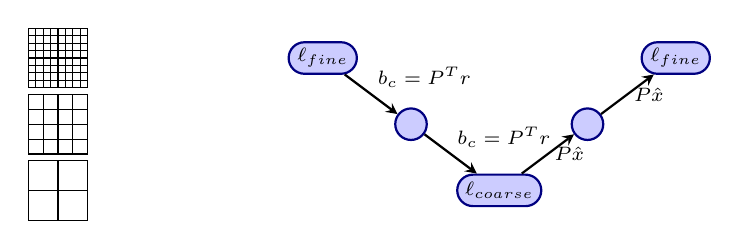
\begin{tikzpicture}
        [>=stealth,
        every node/.style={inner sep=2pt},
        restrict/.style={thick},
        prolong/.style={thick},
        mglevel/.style={rounded rectangle,draw=blue!50!black,fill=blue!20,thick,minimum size=4mm},
        ]
        \begin{scope}\scriptsize
          \newcommand\mgdx{4.0em}
          \newcommand\mgdy{3.0em}
          \newcommand\mgl[1]{(pow(2,#1+1))}
          \newcommand\mgloc[4]{(#1 + #4*\mgdx*#3,#2 + \mgdy*#3)}
          \node[mglevel] (down0) at \mgloc{0}{0}{2}{-1} {\mglevel$_{fine}$};
          \node[mglevel] (down1) at \mgloc{0}{0}{1}{-1} {};
          \node[mglevel] (coarse) at \mgloc{0}{0}{0}{-1} {\mglevel$_{coarse}$};

          \node[mglevel] (up1) at \mgloc{0}{0}{1}{1} {};
          \node[mglevel] (up0) at \mgloc{0}{0}{2}{1} {\mglevel$_{fine}$};

          \path[->,restrict] (down0) edge node [above right] {$b_c = P^T r$} (down1)
          (down1) edge node [above right] {$b_c = P^T r$} (coarse);

          \path[->,prolong] (coarse) edge node [right] {$P \hat x$} (up1)
          (up1) edge node [right] {$P \hat x$} (up0);

          % grids
          \newcommand\mghx{0.9*\mgdx}
          \newcommand\mghy{0.9*\mgdy}

          \draw[shift=\mgloc{-5*\mgdx}{0}{2}{0},
          xstep=\mghy/\mgl{2},
          ystep=\mghy/\mgl{2}]
          (-0.5*\mghy,-0.5*\mghy) grid (0.5*\mghy,0.5*\mghy);

          \draw[shift=\mgloc{-5*\mgdx}{0}{1}{0},
          xstep=\mghy/\mgl{1},
          ystep=\mghy/\mgl{1}]
          (-0.5*\mghy,-0.5*\mghy) grid (0.5*\mghy,0.5*\mghy);

          \draw[shift=\mgloc{-5*\mgdx}{0}{0}{0},
          xstep=\mghy/\mgl{0},
          ystep=\mghy/\mgl{0}]
          (-0.5*\mghy,-0.5*\mghy) grid (0.5*\mghy,0.5*\mghy);
        \end{scope}
      \end{tikzpicture}
      \label{fig:MG}
    \end{figure}
  \end{itemize}
\end{frame}

\begin{frame}{Aggregation and coarsening}
  \begin{figure}
    \centering
    \includegraphics[width=0.4\textwidth]{figures/MG/LubyAgg1} \qquad \qquad
    \includegraphics[width=0.4\textwidth]{figures/MG/LubyAgg2} 
    \caption{$MIS(2)$ finds root nodes (red), defines aggregates, contraction $T$.}
  \end{figure}

  \begin{figure}
    \centering
    \includegraphics[width=0.4\textwidth]{figures/MG/CoarseUnsmoothedRoot} \qquad \qquad
    \includegraphics[width=0.4\textwidth]{figures/MG/CoarseSmoothedRoot}
    \caption{Coarse graph: unsmoothed $T^T A T$, smoothed $P^T A P = (ST)^T A (ST)$.}
  \end{figure}
\end{frame}

\begin{frame}{Fine-grained parallelism for setup}
  \begin{itemize}
  \item SpMM: Sparse matrix-matrix products
    \begin{enumerate}
    \item $P = S T = (1 - \omega D^{-1}A) T$
    \item $A P$
    \item $P^T (A P) = R (A P)$
    \end{enumerate}
  \item Three GPU phases to SpMM: Expand, Sort, Contract
  \item Pros of ESC
    \begin{itemize}
    \item Low memory usage per thread
    \item High-level primitives
    \item Predictable performance
    \end{itemize}
  \item Cons of ESC
    \begin{itemize}
    \item Large global memory usage, can be hard to predict
    \item High bandwidth to global memory
    \item Multiplications and additions in separate phases---no FMA
    \end{itemize}
  \end{itemize}
\end{frame}

\begin{frame}{Fine-grained parallelism in SpMM}
  \begin{figure}
    \centering
    \includegraphics[width=0.8\textwidth]{figures/MG/SACUSPExpand}
  \end{figure}
  \begin{itemize}
  \item Enumerate all scalar products contributing to row of product, $\hat C$
  \item Implemented using \texttt{scan} and \texttt{gather}
  \item Radix sort contributions to each row (two calls to \texttt{sort})
  \item Contract row: \texttt{reduce\_by\_key}
  \end{itemize}
\end{frame}

\begin{frame}{Sorting optimization and performance}
  \begin{itemize}
  \item Sorting optimization, similar to B40C (Merrill and Grimshaw, 2011)
    \begin{itemize}
    \item Bin expanded rows ($\hat C$) by length
    \item Short rows: single thread via optimal sorting network
    \item Medium-length: radix sort within block (shared memory)
    \item Long rows: radix sort in global memory
    \end{itemize}
  \end{itemize}
  \begin{figure}
    \centering
    \includegraphics[width=0.5\textwidth]{figures/MG/SACUSPMaticesFE.png}
    \caption{Time to compute $AP$ (ms) on Tesla C2075 and {\bf speedup}.}
  \end{figure}
\end{frame}

\begin{frame}{CUSP Performance summary}
  \begin{figure}
    \centering
    \includegraphics[width=0.8\textwidth]{figures/MG/SACUSPSpeedupAP}
  \end{figure}  
  \begin{itemize}
  \item New CUSP SpMM is faster than CUSPARSE for all test matrices.
  \item Sorting optimization faster except for very irregular graph.
  \end{itemize}
\end{frame}


\begin{frame}{Memory overhead from expansion}
  \begin{figure}
    \centering
    \includegraphics[width=0.48\textwidth]{figures/MG/SACUSPExpansionFactor} \quad
    \includegraphics[width=0.48\textwidth]{figures/MG/SACUSPContractionFactor}
    \caption{Scalar Poisson: Expansion factor $nnz(\hat C)/nnz(A)$, contraction $nnz(\hat C)/nnz(C)$}
  \end{figure}
  \vspace{-2em}
  \begin{itemize}
  \item 3D has much higher variability by row
  \item For elasticity, expansion factor is larger by 3x (for 3D)
  \item Implementation could batch to limit total memory usage
  \end{itemize}  
\end{frame}

\begin{frame}{Memory Streaming Efficiency (GB/Joule)}
  \begin{figure}
    \centering
    \includegraphics<1>[width=0.9\textwidth]{figures/hardware/mem-bandwidth-per-watt}
    \includegraphics<2->[width=0.9\textwidth]{figures/hardware/mem-bandwidth-per-watt-with-host}
  \end{figure}
  \begin{itemize}
  \item<2-> Include 100 W host CPU paired with each GPU device
  \item<3> Implications for SpMM
    \begin{itemize}
    \item Expand-Sort-Compress: multiple accesses to expanded representation
    \item Compare to CPU: no expanded representation, only accessed once
    \end{itemize}
  \end{itemize}
\end{frame}

\begin{frame}{Distributed memory SpMM}
  \begin{figure}
    \centering
    \includegraphics[width=0.6\textwidth]{figures/Mat/parallelSparseMatrix}
  \end{figure}
  \begin{itemize}
  \item Matrices $A$ and $P$ partitioned by rows
  \item Stored as $P_{\text{rank}} = [\hat P_d, \hat P_o]_{\text{rank}}$, map $\hat p$: local $\hat P_o$ to global col
  \item CPU: unpack off-process rows $\check P_{\text{rank}} = [\check P_d, \check P_o]_{\text{rank}}$
    \begin{equation*}
      \begin{bmatrix}
        AP = \widehat{AP}_d & \widehat{AP}_o
      \end{bmatrix}
      =
      \begin{bmatrix}
        \hat A_d & \hat A_o
      \end{bmatrix}
      \begin{bmatrix}
        \hat P_d & \alert<2>{\hat P_o} \\
        \check P_d & \alert<2>{\check P_o}
      \end{bmatrix}
    \end{equation*}
  \item<2-> \alert<2>{$\hat P_o$ and $\check P_o$ have different column spaces (defined by $\hat p$ and $\check p$).}
  \item<3> GPU: Global column okay with GPU (already sorting); all of $\check P$ must be transferred
  \end{itemize}
\end{frame}

\section{Versatility}

\begin{frame}{Versatility of accelerators for multiphysics engineering/science}
  \begin{itemize}
  \item Library implementations for different sizes
  \item Do not want to recompile for every model variant
    \begin{itemize}
    \item Provenance/reproducibility, testing, build system complexity
    \item Many variants used simultaneously in same application
    \item Model changes in optimization loop, large state to carry to next iteration
    \end{itemize}
  \item Material and chemistry libraries: high variability, multiphysics
    \begin{itemize}
    \item 5-3000 chemical species, crystal grains, energy groups, etc
    \item 5-10000 flops for equation of state (humidity, combustion, ionization)
      \begin{itemize}
      \item Defined implicitly: need local Newton iteration to evaluate (convergence test)
      \end{itemize}
    \item Modified constantly by domain scientists (not software engineers)
    \end{itemize}
  \item Do not need optimality in all cases, should degrade \emph{gracefully}
    \begin{itemize}
    \item Warp size, number of registers, shared memory size
    \item Data dependencies/convergence irregularity at quadrature points
    \item Memory reuse conflicts with vectorization
    \end{itemize}
  \end{itemize}
\end{frame}

\begin{frame}{Example: Climate}
  \begin{itemize}
  \item Many chemical species: $\sim 100$ atmosphere, $\sim 20$ ocean
  \item Users change reaction mechanisms and selected tracers
  \item Tridiagonal solves pervasive due to stiffness in vertical (logarithmic depth)
  \item Complicated equations of state: 32-term rational powers and exponentials
  \item Constant turn-around time desired as resolution is increased
    \begin{itemize}
    \item CFL condition: $\Delta t \sim \Delta x$
    \item 2x resolution requires steps/second to double
    \item Already need 1000 steps/second
    \end{itemize}
  \item Different code components maintained by different science teams
  \end{itemize}
\end{frame}

\begin{frame}{Where we are now: $QR$ factorization with MKL on MIC}
  \begin{figure}
    \centering
    \includegraphics[width=\textwidth]{figures/hardware/MKL-dgeqrf-MIC}
  \end{figure}
  \begin{itemize}
  \item Figure compares two CPU sockets (230W TDP) to one MIC (300W TDP plus host)
  \item Performance/Watt only breaks even at largest problem sizes
  \item $10^4 \times 10^4$ matrix takes 667 GFlops: about 2 seconds
  \item MIC cannot strong scale, no more energy efficient/cost effective
  \end{itemize}
\end{frame}

\begin{frame}{Where are we now: latencies (c/o Karl Rupp)}
  \begin{figure}
    \centering
    \includegraphics[width=0.8\textwidth]{figures/hardware/karlrupp-vector-timings-7}
  \end{figure}
  \vspace{-1em}
  \begin{itemize}
  \item GPU: kernel launch overhead of 10--20 $\mu$s
  \item OpenCL toolchain for MIC is atrocious
  \item MIC latencies with OpenMP are decent
  \end{itemize}
\end{frame}

\begin{frame}{\texttt{MPI\_Allreduce} performance, c/o Paul Fischer}
  \includegraphics[width=\textwidth]{figures/hardware/FischerBGQAllReduce.png}
\end{frame}

\begin{frame}\LARGE
  \begin{itemize}
  \item Maximize science per Watt
  \item Versatility is critical for engineering and science
  \item Huge scope remains at problem formulation
  \item Raise level of abstraction at which a problem is formally specified
  \item Algorithmic optimality is crucial
  \end{itemize}
\end{frame}

\end{document}
